\documentclass[runningheads,11pt]{llncs}

\usepackage[T1]{fontenc}
\usepackage{lmodern}
\usepackage{amsmath,amssymb}
\usepackage{booktabs}
\usepackage{array}
\usepackage{tikz}
\usetikzlibrary{arrows.meta}
\usepackage[hidelinks]{hyperref}

\DeclareUrlCommand\file{\urlstyle{tt}}
\newcommand{\efxz}{\texorpdfstring{\mbox{EFX$_0$}}{EFX0}}
\newcommand{\NA}{\mathit{NA}}
\newcommand{\st}{\mathrel{:}}
\newcommand{\Dp}{D^{+}}
\newcommand{\DE}{\textup{DE}}

\begin{document}

\title{\efxz{} Allocations with at Most Three Relevant Goods: A Short Proof by Exchange Cycles}
\titlerunning{\efxz{} with at Most Three Relevant Goods: A Short Proof}

\author{Evan Lin}
\authorrunning{E. Lin}
\institute{University of Illinois Urbana-Champaign}

\maketitle

\begin{abstract}
An allocation of indivisible goods is \efxz{} if no agent envies another agent's bundle after removing any single good from it, even one the envious agent values at zero. We give a short proof that every instance with nonnegative additive valuations in which each agent positively values at most three goods has a complete \efxz{} allocation, in which moreover all bundles but at most one have at most two goods, and a polynomial-time algorithm, Draft and Exchange (\DE{}), that computes one with at most $4n$ exchanges. The heart of the proof is an \emph{Improvement Lemma}: a valid state from which no free agent can absorb the leftover goods is Pareto-dominated by another valid state, reached by one exchange along a cycle or a path of agents. The proof, derived independently twice and refereed once with no error found (by an independent AI agent; there has been no human peer review), is machine-checked in Lean, together with the algorithm, its bound of $4n$ exchanges and its running time $O(n(n+m))$; it was also checked by computer on millions of states.
\keywords{Fair division \and Indivisible goods \and EFX \and Exchange cycles}
\end{abstract}

\section{Introduction}\label{sec:intro}

Agents $N$ ($|N|=n\ge1$) share a set $M$ of $m$ indivisible goods with nonnegative additive valuations $v_i(S)=\sum_{g\in S}v_i(g)$. An allocation $X$ assigns every good to exactly one agent, who receives the bundle $X_i$; no good is left out (allocations are \emph{complete}). It is \emph{\efxz{}} if
\[
  v_i(X_i)\ \ge\ v_i(X_j\setminus\{h\})\qquad\text{for all } i\ne j \text{ and all } h\in X_j,
\]
and \emph{EFX} asks this only for goods $h$ with $v_i(h)>0$~\cite{AmanatidisBFV22}. So \efxz{} implies EFX, and the two coincide for positive values. \emph{Under \efxz{}, if $X_j$ contains a good that $i$ values at $0$, then $i$ must not envy $X_j$ at all.} Whether complete EFX allocations always exist for additive valuations is open; they are known to exist in special cases, among them three agents~\cite{ChaudhuryGM20} or three types~\cite{HVGNV25}, $m\le n+3$~\cite{Mahara21}, four agents and at most nine goods~\cite{AlkassarFM26}, goods valued by at most two agents~\cite{AfshinmehrAMMS26,ChristodoulouFKS23,SgouritsaS25,KavianiSS24}, and hypergraphs of girth at least four~\cite{LianeasSS26} (Table~\ref{tab:rw} in Appendix~\ref{app:rw}). Let $R_i=\{g\st v_i(g)>0\}$. If $|R_i|\le2$ for all $i$, serial dictatorship gives \efxz{}~\cite{MrdEfx}. For $|R_i|\le4$, Viswanathan and Mehta~\cite{ViswanathanM24} announce ordinary EFX, with a proof sketch; their algorithm gives the goods nobody values to an arbitrary agent, which can break \efxz{}.

\begin{theorem}[existence and shape]\label{thm:main}
Every instance with $n\ge1$ agents and nonnegative additive valuations in which every agent positively values at most three goods has a complete \efxz{} allocation in which all bundles but at most one have at most two goods. In particular this holds when every agent values exactly three goods and is \emph{balanced} (values none of them more than the other two together).
\end{theorem}

\begin{theorem}[algorithm]\label{thm:algo}
Algorithm \DE{} (Section~\ref{sec:algo}) computes such an allocation with at most $n$ peeling steps and at most $4n$ exchanges, each taking time polynomial in $n$ and $m$; on real values, a comparison of two sums of at most two values of one agent counts as one step.
\end{theorem}

\paragraph{Status.} The core of the proof, the Improvement Lemma (Theorem~\ref{thm:improve}), was derived independently twice, by two different arguments~\cite{Repo}. It was refereed once, with no error found, by an independent AI agent (a separate session of our coding assistant, given only the written proof); there has been no human peer review. Every step has been checked by computer as described in Section~\ref{sec:evidence}. The Improvement Lemma, soundness (Theorem~\ref{thm:sound}), \DE{} with at most $4n$ exchanges and its running time, the shape and the appendices' results are machine-checked in Lean~4, also for ordered values. A long version with every proof in the body, a worked example with a figure, and pseudocode is \file{paper/k3-simple/long.pdf} in~\cite{Repo}.

\section{Preliminaries}\label{sec:prelim}

The \emph{threat} of a nonempty set $B$ to agent $i$ is $\theta_i(B)=v_i(B)-\min_{h\in B}v_i(h)$, and $\theta_i(\emptyset)=0$; agent $i$ is \emph{safe} in $X$ if $v_i(X_i)\ge\theta_i(X_j)$ for all $j\ne i$, so $X$ is \efxz{} iff every agent is safe. A good is \emph{alone} if it is the only good of its bundle. When $|R_i|=3$, we name $i$'s goods so that $v_i(a_i)\ge v_i(b_i)\ge v_i(c_i)>0$, ties broken by index, and write $a_i\succ_ib_i\succ_ic_i$. Agent $i$ is \emph{balanced} if $v_i(a_i)\le v_i(b_i)+v_i(c_i)$, \emph{strictly} if the inequality is strict. Proofs of this section are in Appendix~\ref{app:prelim}.

\begin{lemma}[threats]\label{lem:threat}
(a) $\theta_i(B)=0$ if $|B|\le1$; (b) $\theta_i(B)\le v_i(B\cap R_i)$; (c) $\theta_i(\{g,h\})=\max(v_i(g),v_i(h))$.
\end{lemma}

\begin{lemma}[safety]\label{lem:safe}
Let $i$ be balanced with $|R_i|=3$, and $X$ an allocation. (a) If $b_i,c_i\in X_i$, $i$ is safe. (b) Let $y\in X_i\cap R_i$ or $y=\bot$, and $G_y=\{g\in R_i\st g\succ_iy\}$ ($G_\bot=R_i$). If no bundle $X_j$, $j\ne i$, $|X_j|\ge2$, contains a good of $G_y$, then $i$ is safe, unless $y=a_i$ and some $X_j$, $j\ne i$, $|X_j|\ge3$, contains $b_i$ and $c_i$.
\end{lemma}

\begin{lemma}[peeling]\label{lem:peel}
Let $i\in N$ and $P\subseteq M$ with $|P|\le1$ and $v_i(P)\ge v_i(M\setminus P)$. If the instance without $i$ and $P$ has an \efxz{} allocation $Z$, then $Z$ with $X_i=P$ is \efxz{}.
\end{lemma}

\noindent\emph{Rule R1}: with $G$ the remaining goods and $p$ agent $i$'s favourite good of $G$, agent $i$ leaves with $P=\emptyset$ if it values no good of $G$, and with $P=\{p\}$ if $v_i(G\setminus\{p\})\le v_i(p)$.

\begin{lemma}[when R1 applies to nobody]\label{lem:R1fail}
If $i$ values at most three goods of $G$ and R1 does not apply to $i$, then $i$ values exactly three goods of $G$ and is strictly balanced with respect to them.
\end{lemma}

\section{States and Soundness}\label{sec:states}

In the \emph{core case} every agent values exactly three goods and is strictly balanced; goods valued by nobody may exist.
A \emph{state} $Y$ gives each agent $i$ a holding $Y_i\in\{\emptyset,\{a_i\},\{b_i\},\{c_i\},\{b_i,c_i\}\}$, pairwise disjoint. $U$ is the set of \emph{pair holders} ($Y_i=\{b_i,c_i\}$); $J=M\setminus\bigcup_iY_i$ is the set of \emph{leftover} goods; for $i\notin U$ with $|Y_i|=1$ we write $Y_i=\{y_i\}$. The \emph{utility} $u_i(Y)$ is $4,3,2,1,0$ for the pair, $\{a_i\}$, $\{b_i\}$, $\{c_i\}$, $\emptyset$; $Y'$ \emph{Pareto-dominates} $Y$ if $u_i(Y')\ge u_i(Y)$ for all $i$, strictly for some $i$.
\begin{itemize}
\item The \emph{needs} are $N_i=\emptyset$ for $i\in U$, $N_i=R_i$ if $Y_i=\emptyset$, and $N_i=\{g\in R_i\st g\succ_iy_i\}$ otherwise; $\NA=\bigcup_iN_i$. No agent needs its own good. ($N$ is the set of agents; $N_i$, with a subscript, are the needs of agent $i$.)
\item $Y$ is \emph{valid} if every $g\in\NA$ is the only good of some agent ($Y_j=\{g\}$; then $j\notin U$).
\item An agent $i\notin U$ is \emph{free} if $Y_i=\emptyset$ or $y_i\notin\NA$; $F$ is the set of free agents.
\item The \emph{need digraph} $D$ has the agents outside $U$ as vertices and an arc $j\to j'$ when $j$ holds a single good $y_j\in N_{j'}$. It has no loops.
\item Agent $x$ is \emph{exposed} for $o$ if $x\ne o$, $x\notin U$, $Y_x=\{a_x\}$ and $b_x,c_x\in J\cup Y_o$; $E_o$ is the set of these agents.
\item Agent $o$ is a \emph{valid absorber} with set $H$ if $o\in F\cup U$, (A1) $\{b_x,c_x\}\cap J\ne\emptyset$ for every $x\in E_o$, and (A2) $H\subseteq J$ meets every $\{b_x,c_x\}\cap J$ ($x\in E_o$) and $|H|\le|F\setminus\{o\}|$. $Y$ is \emph{completable} if some agent is a valid absorber.
\item The \emph{completion} with $o$ and $H$: each good of $H$ goes to a different free agent other than $o$; $o$ receives $X_o=Y_o\cup(J\setminus H)$; every other agent $i$ keeps $X_i=Y_i$, or $X_i=Y_i\cup\{h\}$ if it received $h\in H$.
\end{itemize}

\begin{theorem}[soundness]\label{thm:sound}
If $Y$ is valid and $o$ is a valid absorber with set $H$, the completion is \efxz{}, and only $X_o$ can have more than two goods.
\end{theorem}

\noindent The proof (Appendix~\ref{app:sound}) shows that needed goods stay alone, and that no agent $x\ne o$, $x\notin U$, holding only $a_x$ finds $b_x$ and $c_x$ in $X_o$: otherwise $b_x,c_x\in J\cup Y_o$, so $x\in E_o$, and $H$ took one of them out of $X_o$. Lemma~\ref{lem:safe} then applies to every agent.

\begin{lemma}\label{lem:basic}
(Draft) If the agents, in any order, each take the first of $a_i,b_i,c_i$ not yet taken (or nothing), the result is a valid state. Now let $Y$ be valid and $Y'$ a state. (F1) If $u_i(Y')\ge u_i(Y)$, then $N'_i\subseteq N_i$. (F2) Every agent outside $U\cup F$ has an out-arc in $D$. (Transfer) If a state $Y'$ has $u_i(Y')\ge u_i(Y)$ for all $i$, strictly for some, and every $g\in\NA$ is the only good of some agent in $Y'$, then $Y'$ is valid and Pareto-dominates $Y$.
\end{lemma}

\begin{proof}
(Draft) A good that $i$ needs was taken before $i$'s turn, alone, by an earlier agent, and holdings do not change. (F1) If $Y'_i$ is the pair, $N'_i=\emptyset$; if $Y'_i=\{g'\}$, then $Y_i$ is $\emptyset$ or a single good ranked at most as high as $g'$, so every good ranked above $g'$ is in $N_i$; if $Y'_i=\emptyset$, then $Y_i=\emptyset$. (F2) Such a $j$ holds $y_j\in\NA$, so some $j'$ needs $y_j$; $j'\ne j$, and $j'\notin U$ since pair holders need nothing. (Transfer) By (F1), $\NA'\subseteq\NA$. \qed
\end{proof}

\section{The Improvement Lemma}\label{sec:improve}

\begin{theorem}[Improvement Lemma]\label{thm:improve}
In the core case, let $Y$ be valid, with no free agent a valid absorber and some agent not in $U$. Then some valid state Pareto-dominates $Y$, obtained by one need cycle, pair chain or exchange cycle, found in polynomial time.
\end{theorem}

\noindent If $Y$ is not completable, the hypotheses hold (if $U=N$, every agent is a valid absorber with $H=\emptyset$, as exposed agents are outside $U$). So every valid state that no valid state dominates is completable. In the proof, $Y$ is valid.

\begin{lemma}[need cycle; pair chain]\label{lem:P}
(a) If $D$ has a cycle, $Y$ is dominated by a valid state. (b) If some $x\notin U$ has $Y_x=\{a_x\}$ and $b_x,c_x\in J$, $Y$ is dominated by a valid state.
\end{lemma}

\begin{proof}
(a) Let $j_0\to\dots\to j_{k-1}\to j_0$ be a cycle ($k\ge2$); its agents hold single goods. Let each $j_{t+1}$ take $y_{j_t}$ (indices mod $k$). The goods are permuted, each $j_{t+1}$ receives a good it needs, and a needed good held by $j_t$ is now held alone by $j_{t+1}$; others are unchanged. Transfer applies.
(b) Walk $j_0=x$, $j_{t+1}=$ an out-neighbour of $j_t$, while one exists. A repeat gives a cycle: use (a). Otherwise the walk stops at $j_k$ with no out-arc. Let $x$ take $\{b_x,c_x\}$ and $j_t$ take $y_{j_{t-1}}$ for $1\le t\le k$ ($y_{j_0}=a_x$); the old good of $j_k$, if any, becomes leftover. Holdings stay disjoint ($b_x,c_x$ were leftover), $x$ goes from $3$ to $4$, and each $j_t$, $t\ge1$, gets a needed good. Leftover goods are not needed (validity); $y_{j_t}$ ($t<k$) moves to $j_{t+1}$ alone; and $j_k\notin U$ has no out-arc, so $j_k\in F$ by (F2) and its old good is not needed. Transfer applies. \qed
\end{proof}

\noindent From now on assume \textbf{(P)}: no $x\notin U$ with $Y_x=\{a_x\}$ has $b_x,c_x\in J$.

\begin{lemma}\label{lem:free}
Assume (P). (a) If $o\in F$ holds nothing, $E_o=\emptyset$ and $o$ is a valid absorber with $H=\emptyset$. (b) If $o\in F$ holds $y_o$, every $x\in E_o$ has $\{b_x,c_x\}=\{y_o,h_x\}$ with $h_x\in J$; with $H_o=\{h_x\st x\in E_o\}$, $o$ is a valid absorber iff $|H_o|\le|F|-1$, and then with $H=H_o$. (c) An agent $x$ lies in $E_o$ for at most one free $o$ holding a good, so $h_x$ depends only on $x$. (d) If $F=\emptyset$ and $U\ne N$, $D$ has a cycle.
\end{lemma}

\begin{proof}
(a) $x\in E_o$ would have $b_x,c_x\in J$, against (P). (b) $b_x,c_x\in J\cup\{y_o\}$, not both in $J$, and $b_x\ne c_x$; so one is $y_o$ and the other is leftover. Then $\{b_x,c_x\}\cap J=\{h_x\}$, and $H$ meets all of these iff $H\supseteq H_o$; and $|F\setminus\{o\}|=|F|-1$. (c) If $x\in E_o\cap E_{o'}$, $o\ne o'$, then $\{b_x,c_x\}=\{y_o,y_{o'}\}$ has no leftover good, against (b). (d) Every agent outside $U$ has an out-arc by (F2), and there is one. \qed
\end{proof}

\noindent The \emph{exchange digraph} $\Dp$ (under (P)) adds to $D$ an \emph{exposure arc} $o\to x$, labelled $h_x$, for every $o\in F$ holding a good and every $x\in E_o$. Heads of exposure arcs hold their tops and need nothing; heads of need arcs need a good; so the head determines the kind of arc. The \emph{exchange} along a cycle $(w_0,\dots,w_{k-1})$ of $\Dp$ ($k\ge2$, indices mod $k$) lets $w_{t+1}$ take its pair $\{y_{w_t},h_{w_{t+1}}\}$ if $w_t\to w_{t+1}$ is an exposure arc, and $y_{w_t}$ alone if it is a need arc; agents off the cycle keep their holdings. Every cycle agent holds a single good and has one predecessor, so this is well defined.

\begin{lemma}[exchange cycle]\label{lem:exchange}
Assume (P). If the exposure arcs of a cycle $C$ of $\Dp$ have distinct labels, the exchange along $C$ is valid and Pareto-dominates $Y$; its new pair holders are the heads of the exposure arcs.
\end{lemma}

\begin{proof}
Each $y_{w_t}$ moves to $w_{t+1}$ only; the labels are leftover and distinct; agents off $C$ keep other goods. So holdings are disjoint. Exposure heads go from $3$ to $4$; need heads receive a needed good; others are unchanged. If $g\in\NA$ is held by $j$ alone and $j=w_t\in C$, then $w_t\notin F$, so $w_t\to w_{t+1}$ is a need arc and $w_{t+1}$ holds $g$ alone; if $j\notin C$, $j$ keeps $g$. Transfer applies. \qed
\end{proof}

\begin{lemma}[an exchange cycle exists]\label{lem:cycle}
Assume (P), $F\ne\emptyset$, no free agent holds nothing, and $|H_o|\ge|F|$ for all $o\in F$. Then $\Dp$ has a cycle whose exposure arcs have distinct labels.
\end{lemma}

\begin{proof}
List $F=\{o_1,\dots,o_f\}$ and pick $q_{o_i}\in H_{o_i}\setminus\{q_{o_1},\dots,q_{o_{i-1}}\}$, possible since $|H_{o_i}|\ge f>i-1$. Let $x_{o}\in E_{o}$ have protecting good $q_{o}$. Define $\sigma(o)=x_o$ for $o\in F$, and $\sigma(j)=$ an out-neighbour in $D$ for $j\notin U\cup F$ (F2). Then $\sigma(j)\notin U$, $\sigma(j)\ne j$, and $j\to\sigma(j)$ is an arc of $\Dp$. Iterating $\sigma$ from any agent outside $U$ repeats an agent and gives a cycle; its exposure arcs $o\to x_o$ carry the distinct labels $h_o$. \qed
\end{proof}

\begin{proof}[of Theorem~\ref{thm:improve}]
If (P) fails, Lemma~\ref{lem:P}(b). If $F=\emptyset$, Lemma~\ref{lem:free}(d) gives a cycle of $D$, and Lemma~\ref{lem:P}(a). Otherwise no free agent absorbs, so none holds nothing and $|H_o|\ge|F|$ for all $o\in F$ (Lemma~\ref{lem:free}(a,b)); Lemmas~\ref{lem:cycle} and~\ref{lem:exchange}. Each step is a walk or a greedy choice. \qed
\end{proof}

\section{The Algorithm Draft and Exchange}\label{sec:algo}

\noindent\rule{\textwidth}{0.4pt}\par
\noindent\textbf{Algorithm \DE{}.} \textbf{1. Peel.} While at least two agents remain and rule R1 applies to one of them, it leaves with its set $P$. If one agent remains, it takes all remaining goods; stop. \textbf{2. Draft.} The remaining agents, in index order, take the first of $a_i,b_i,c_i$ not yet taken, or nothing. \textbf{3. Exchange.} Repeat: if (P) fails, apply the pair chain (or need cycle) of Lemma~\ref{lem:P}(b); else, if every agent holds its pair, or a free agent holds nothing, or a free $o$ has $|H_o|\le|F|-1$, stop with that absorber (any agent if all hold pairs; $H=\emptyset$, $\emptyset$, $H_o$ respectively); else, if $F=\emptyset$, apply a need cycle; else apply the exchange cycle of Lemma~\ref{lem:cycle}. \textbf{4. Complete} with the absorber $o$ and $H$.\par
\noindent\rule{\textwidth}{0.4pt}

\begin{theorem}\label{thm:de}
On every instance with $|R_i|\le3$ for all $i$, \DE{} returns a complete \efxz{} allocation in which all bundles but at most one have at most two goods, after at most $n$ peels and $4n$ exchanges.
\end{theorem}

\begin{proof}
By Lemma~\ref{lem:peel} and induction on the peels, it suffices that the allocation of the residual instance is \efxz{}; with one agent this is trivial. Otherwise, by Lemma~\ref{lem:R1fail}, we are in the core case. The draft is valid (Lemma~\ref{lem:basic}). Each exchange keeps validity and raises $\sum_iu_i\in[0,4n]$ by at least $1$ (Lemmas~\ref{lem:P}, \ref{lem:free}(d), \ref{lem:exchange}, \ref{lem:cycle}, as in the proof of Theorem~\ref{thm:improve}), so there are at most $4n$. At the stop, $o$ is a valid absorber with $H$ (Lemma~\ref{lem:free}, or, if every agent holds its pair, the remark after Theorem~\ref{thm:improve}), and the completion is \efxz{} with only $X_o$ large (Theorem~\ref{thm:sound}). Peeled agents get at most one good. \qed
\end{proof}

\noindent Theorems~\ref{thm:main} and~\ref{thm:algo} follow; each iteration needs one pass over agents and goods, so \DE{} takes $O(n(n+m))$ steps, input included (Lean-checked; on real values, in the comparison model of Section~\ref{sec:intro}). The absorber test is applied only under (P), where it is a count; in general it would ask for a smallest hitting set.

\paragraph{Example.} Goods $g_0,\dots,g_9$; agents $x_1$, $x_1'$, $x_2$, $x_2'$, $o_1$, $o_2$ rank $(g_0,g_4,g_6)$, $(g_1,g_4,g_7)$, $(g_2,g_5,g_8)$, $(g_3,g_5,g_9)$, $(g_2,g_3,g_4)$, $(g_0,g_1,g_5)$ (values $4,3,2$, say). Nobody is peeled; the draft gives the $x$'s their tops, $o_1$ its $c=g_4$ and $o_2$ its $c=g_5$. Then $\NA=\{g_0,\dots,g_3\}$, $J=\{g_6,\dots,g_9\}$, $F=\{o_1,o_2\}$, $H_{o_1}=\{g_6,g_7\}$ (from $x_1,x_1'$) and $H_{o_2}=\{g_8,g_9\}$: no free agent absorbs. There is no need cycle, pair chain, or cycle of $\Dp$ with one exposure arc, and each of the four valid states that dominate this one gives pairs to two agents. \DE{} picks $q_{o_1}=g_6$, $q_{o_2}=g_8$ and exchanges along $o_1\to x_1\to o_2\to x_2\to o_1$ (Figure~\ref{fig:cycle}): $x_1$ takes $\{g_4,g_6\}$, $o_2$ takes $g_0$, $x_2$ takes $\{g_5,g_8\}$, $o_1$ takes $g_2$. Now $\NA=\emptyset$, $J=\{g_7,g_9\}$, and $x_1'$ absorbs with $H=\emptyset$: $X_{x_1'}=\{g_1,g_7,g_9\}$, an \efxz{} allocation. Every Pareto improvement there gives pairs to two agents at once, so a search that applies one short move at a time gets stuck. A state with no free absorber and no such short move needs $n\ge6$ and $m\ge8$, both attained (a written proof, not refereed), and on a family of rings every exchange cycle needed $k$ exposure arcs in our computations for $k\le5$ (not proved; Appendix~\ref{app:short}).

\begin{figure}[t]
\centering
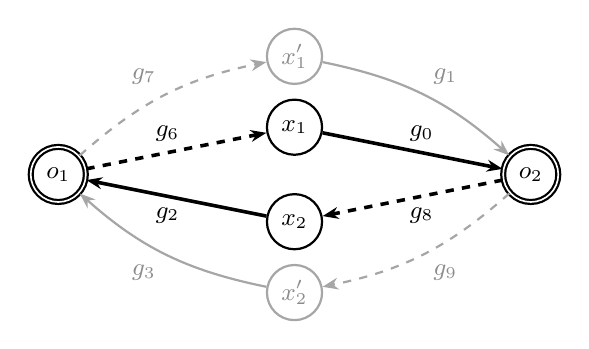
\begin{tikzpicture}[font=\small, ag/.style={draw, thick, circle, minimum size=7mm, inner sep=1pt},
  fr/.style={draw, thick, circle, double, minimum size=7mm, inner sep=1pt},
  need/.style={-{Stealth[length=2mm]}, thick}, expo/.style={-{Stealth[length=2mm]}, thick, dashed},
  off/.style={draw=black!35, text=black!45}]
\node[fr] (o1) at (0,0) {$o_1$}; \node[fr] (o2) at (6,0) {$o_2$};
\node[ag] (x1) at (3,0.6) {$x_1$}; \node[ag, off] (x1p) at (3,1.5) {$x_1'$};
\node[ag] (x2) at (3,-0.6) {$x_2$}; \node[ag, off] (x2p) at (3,-1.5) {$x_2'$};
\draw[expo, line width=1.3pt] (o1) -- node[above, pos=0.45]{$g_6$} (x1);
\draw[need, line width=1.3pt] (x1) -- node[above, pos=0.55]{$g_0$} (o2);
\draw[expo, line width=1.3pt] (o2) -- node[below, pos=0.45]{$g_8$} (x2);
\draw[need, line width=1.3pt] (x2) -- node[below, pos=0.55]{$g_2$} (o1);
\draw[expo, black!35] (o1) to[bend left=15] node[above left, black!45]{$g_7$} (x1p);
\draw[need, black!35] (x1p) to[bend left=15] node[above right, black!45]{$g_1$} (o2);
\draw[expo, black!35] (o2) to[bend left=15] node[below right, black!45]{$g_9$} (x2p);
\draw[need, black!35] (x2p) to[bend left=15] node[below left, black!45]{$g_3$} (o1);
\end{tikzpicture}
\caption{The exchange digraph of the drafted state of the example. Double circles: free agents. Dashed: exposure arcs (labelled by the protecting good); solid: need arcs (labelled by the good that moves). Black: the cycle chosen by \DE{}.}\label{fig:cycle}
\end{figure}

\section{Verification Status, Evidence and Conclusion}\label{sec:evidence}

The Improvement Lemma, soundness and \DE{} (correctness, shape, at most $4n$ exchanges, peeling included) are machine-checked in Lean~4, also for ordered values, as are the results of Appendices~\ref{app:short} and~\ref{app:limits} (\cite{Repo}, \file{lean/EFX/K3DE*.lean}; standard axioms only; an independent AI referee found the formal statements faithful to the text). The Improvement Lemma was found twice independently: the proof above and a ``rainbow walk'' (\cite{Repo}, \file{k3/simplify/po/hall/NOTES.md} and \file{po/potential/NOTES.md}). One referee, an independent AI agent given only the written proof, found no error (\file{po/referee/README.md}); there has been no human peer review; its four presentation fixes are applied (explicit completion and owner constraint; $h_x$ well defined; Lemma~\ref{lem:P}(a) when $F=\emptyset$; test wording). Three implementations (the two proofs as code, and the referee's, written from the text alone) assert every claim of the proofs, with raw \efxz{} checks of the outputs, on millions of valid states and runs, without failure (Appendix~\ref{app:evidence}). Our script \file{paper/k3-simple/examples/check_examples.py} rechecks every example and runs \DE{}, peeling included, on $40{,}000$ random instances (Appendix~\ref{app:evidence}). The shape cannot be improved in the obvious ways: some core instances need a bundle of three goods, and some need four (Appendix~\ref{app:limits}). \efxz{} with four relevant goods per agent is open (for EFX, see~\cite{ViswanathanM24}); so are a better bound than $4n$ exchanges, and the least size of the large bundle.

\paragraph{Acknowledgments.} The proofs, code and the Lean formalizations were developed with the assistance of AI coding agents (Claude Code); this paper was also drafted with their assistance.

\bibliographystyle{splncs04}
\bibliography{refs}

\clearpage
\appendix

\section{Proofs for Section~\ref{sec:prelim}}\label{app:prelim}

\begin{proof}[of Lemma~\ref{lem:threat}]
(a) $\theta_i(\{h\})=0$. (b) The minimum is at least $0$ and $v_i(B)=v_i(B\cap R_i)$. (c) $v_i(g)+v_i(h)-\min(v_i(g),v_i(h))$. \qed
\end{proof}

\begin{proof}[of Lemma~\ref{lem:safe}]
Fix $j\ne i$; if $|X_j|\le1$, $\theta_i(X_j)=0$. Let $|X_j|\ge2$ and $T=X_j\cap R_i$, so $\theta_i(X_j)\le v_i(T)$. (a) $T\subseteq\{a_i\}$, and $v_i(a_i)\le v_i(b_i)+v_i(c_i)\le v_i(X_i)$. (b) If $y=\bot$, $T\subseteq G_\bot$ is empty. Otherwise each $g\in T$ is neither in $G_y$ nor $y$, so $y\succ_ig$ and $v_i(g)\le v_i(y)\le v_i(X_i)$; this settles $|T|\le1$. If $|T|\ge2$, then $y=a_i$ and $T=\{b_i,c_i\}$; if $|X_j|=2$, $\theta_i(X_j)=v_i(b_i)\le v_i(a_i)$ by Lemma~\ref{lem:threat}(c); if $|X_j|\ge3$ we are in the exception. \qed
\end{proof}

\begin{proof}[of Lemma~\ref{lem:peel}]
Every other bundle lies in $M\setminus P$, so its threat to $i$ is at most $v_i(M\setminus P)\le v_i(P)$. The bundle $P$ has at most one good, so its threat is $0$. Other constraints are those of $Z$. \qed
\end{proof}

\begin{proof}[of Lemma~\ref{lem:R1fail}]
R1 fails, so $v_i(p)>0$ and $v_i(G\setminus\{p\})>v_i(p)$. With at most two valued goods, $v_i(G\setminus\{p\})$ would be the value of at most one good, at most $v_i(p)$. So $i$ values three goods, $p=a_i$, and $v_i(b_i)+v_i(c_i)>v_i(a_i)$. \qed
\end{proof}

\noindent If $|R_i|\le2$ for all agents, serial dictatorship with the last agent taking the rest is \efxz{}: each pick satisfies R1 (Lemma~\ref{lem:peel}, induction).

\section{Proof of Theorem~\ref{thm:sound}}\label{app:sound}

\begin{proof}
\emph{Sizes.} A free agent other than $o$ holds at most one good and receives at most one; a pair holder has two goods; other agents keep one good. So only $X_o$ can have three or more goods.
\emph{(N) Needed goods stay alone.} For $g\in\NA$, validity gives $Y_j=\{g\}$; $j\notin U\cup F$, so $j\ne o$ and $j$ receives no good of $H$; so $X_j=\{g\}$.
\emph{(OC)} No $x\ne o$, $x\notin U$, $Y_x=\{a_x\}$, has $b_x,c_x\in X_o$: otherwise $b_x,c_x\in Y_o\cup J$, so $x\in E_o$, and by (A2) $H$ contains a leftover good of $\{b_x,c_x\}$, which went to another agent and is not in $Y_o$, hence not in $X_o$.
\emph{Safety.} Agents are balanced. If $i\in U$, Lemma~\ref{lem:safe}(a). If $i\notin U$, apply Lemma~\ref{lem:safe}(b) with $y=y_i$ (or $\bot$): $G_y=N_i\subseteq\NA$, so its goods are alone by (N). In the exception, $y_i=a_i$ and $b_i,c_i$ lie in a bundle of at least three goods, which is $X_o$ with $o\ne i$; (OC) excludes this. \qed
\end{proof}

\noindent The proof uses only validity, the definition of a valid absorber, and balance of pair holders.

\section{Short Moves and Large Exchanges}\label{app:short}

A \emph{short move} is a need cycle, a pair chain, or an exchange along a cycle of $\Dp$ with one exposure arc. For example, a \emph{rotation}, in which an agent $k$ exposed for a free agent $r$ takes its pair and its top travels along a need chain to $r$, is a short move.

\begin{proposition}[Lemma~3 of~\cite{Repo}, \file{po/potential/NOTES.md}]\label{prop:short}
In the core case, let $Y$ be valid, with no free valid absorber, $U\ne N$, and no short move. Then $|F|\ge2$, $n\ge6$ and $m\ge8$ (and $n\ge9$, $m\ge12$ if $|F|\ge3$). The bounds $n\ge6$ and $m\ge8$ are attained.
\end{proposition}

\begin{proof}
(P) holds (no pair chain) and $D$ is acyclic (no need cycle), so every walk along need arcs ends at a free agent (F2). By Lemma~\ref{lem:free}, $F\ne\emptyset$, every free agent holds a good, $|H_o|\ge|F|$ for $o\in F$, and the sets $E_o$ are disjoint with $|E_o|\ge|H_o|$. Every agent holds a good. If $F=\{o\}$, some $x\in E_o$ walks along need arcs to $o$, and $o\to x\to\dots\to o$ is a short move. If $F=\{o_1,o_2\}$: walks from $E_{o_1}$ cannot end at $o_1$ (short move), so they end at $o_2$; one of the at least two agents of $E_{o_1}$ is not $o_2$, so a need arc enters $o_2$, $o_2$ needs a good, and $o_2\notin E_{o_1}$. So $E_{o_1}$, and symmetrically $E_{o_2}$, hold at least two non-free agents: $n\ge6$, and $m\ge n+|J|\ge6+2$. If $|F|=k\ge3$, the $E_o$ hold at least $k^2$ agents, at most $k$ of them free: $n\ge k^2$, $m\ge k^2+k$. The example of Section~\ref{sec:algo} has $n=6$; the state with rankings $o_1\colon(g_4,g_5,g_0)$, $o_2\colon(g_6,g_7,g_1)$, $x_1\colon(g_4,g_1,g_2)$, $x_1'\colon(g_5,g_3,g_1)$, $x_2\colon(g_6,g_0,g_2)$, $x_2'\colon(g_7,g_3,g_0)$, where $o_1$ holds $g_0$, $o_2$ holds $g_1$ and the $x$'s their tops, has $n=6$, $m=8$ (checked by our script). \qed
\end{proof}

\noindent In the notes' family of rings with $k$ free agents (each needing the roots of a binary need tree whose leaves are exposed for the previous free agent), every cycle of $\Dp$ has exactly $k$ exposure arcs, and no free agent absorbs iff $k\le2^d$ for trees of depth $d$; both are Lean-checked for every $k$ and $d$.

\section{Limits of the Shape}\label{app:limits}

\begin{lemma}[cases of safety]\label{lem:L5}
Let $R_i=\{a,b,c\}$ with $v_i(a)>v_i(b)>v_i(c)>0$ and $v_i(a)<v_i(b)+v_i(c)$. Agent $i$ is safe in $X$ iff (T) $i$ holds $a$, and also $b$ or $c$, or $b$ and $c$ are not together in a bundle of at least three goods; or (BC) $i$ holds $b$ and $c$; or (B) $i$ holds $b$ and $a$ is alone; or (C) $i$ holds $c$, and $a$ and $b$ are alone; or (E) $a$, $b$, $c$ are all alone.
\end{lemma}

\begin{proof}
Write $x$ for $v_i(x)$: $0<c<b<a<b+c<a+c<a+b<a+b+c$. Let $S=X_i\cap R_i$ and, for $j\ne i$, $T=X_j\cap R_i$; $\theta_i(X_j)$ is $0$ if $T=\emptyset$ or $|X_j|=1$, $v_i(T)$ if $X_j\not\subseteq R_i$, and the larger value if $X_j=T$ has two goods. If $S$ contains $a$ and another good, every threat is at most $b<a+c$: safe (T). If $S=\{b,c\}$, every threat is at most $a<b+c$: safe (BC). If $S=\{a\}$, the threat is $b+c>a$ exactly when $b,c$ share a bundle of at least three goods (it then has a good outside $R_i$), and at most $b$ otherwise: (T). If $S=\{b\}$: if $a$ is not alone its bundle has threat at least $a>b$; if $a$ is alone the remaining threat is at most $c$: (B). If $S=\{c\}$: $a$ must be alone, and $b$ too (its bundle otherwise has threat at least $b>c$): (C). If $S=\emptyset$: any bundle of two or more goods meeting $R_i$ has positive threat: (E). Conversely each case is one of these safe situations. \qed
\end{proof}

\begin{proposition}[limits of the shape]\label{prop:neg}
With values as in Lemma~\ref{lem:L5} for every agent:
(a) if agents $0,1,2$ rank $g_0\succ g_1\succ p_i$, with $p_i$ valued only by $i$, no \efxz{} allocation has all bundles of at most two goods, and $\{g_0\},\{g_1\},\{p_0,p_1,p_2\}$ is \efxz{} in any order;
(b) if agents $0,1,2,3$ rank $g_0\succ g_2\succ p_0$, $g_0\succ g_2\succ p_1$, $g_1\succ g_2\succ p_2$, $g_1\succ g_2\succ p_3$, every \efxz{} allocation has sizes $4,1,1,1$, and one exists.
\end{proposition}

\begin{proof}
(a) Bundles of at most two goods have sizes $2,2,1$: one good is alone. Two agents do not hold $g_0$; (T) fails for them, and (C), (E) need two alone goods; so both are in (BC) or (B) and hold $g_1$: impossible. The stated allocation is (T), (B), (C).
(b) Each top $g_0$, $g_1$ has a different \emph{loser}, an agent ranking it first without holding it. A loser is safe only by (BC) or (B), holding $g_2$, or by (C) or (E), with $g_2$ alone. Both cannot hold $g_2$, so $g_2$ is alone and (BC) is impossible; then each loser needs its top alone too. So $g_0,g_1,g_2$ are alone in three bundles, and the fourth is $\{p_0,\dots,p_3\}$. Giving $g_0,g_2,g_1$ and the $p_i$ to agents $0,1,2,3$ is \efxz{} (cases T, B, T, C). \qed
\end{proof}

\noindent Lemma~\ref{lem:L5} and both parts are Lean-checked for every such valuation; our script confirms them by listing all allocations.

\section{Evidence in Detail}\label{app:evidence}

The tests (\cite{Repo}; \file{k3/simplify/po/hall/}, \file{po/potential/}, \file{po/referee/}) are evidence, not proof; values $4,3,2$ suffice for distinct strictly balanced values by Lemma~\ref{lem:L5}, and the referee also used real values. \emph{First proof as code}: every valid state of every ranking profile with $n=2$ ($m\le6$), $n=3$ ($m\le7$), $n=4$ ($m=5$): $1{,}693{,}750$ states, $269{,}028$ not completable, each improved; $183{,}484$ sampled states; one completion per completable state checked \efxz{}; all $774{,}248$ Pareto-optimal states completable; \DE{}'s loop on $44{,}971$ profiles. \emph{Second proof as code}: about $15.5$ million valid states (every profile with $n=2$, $m\le6$; $n=3$, $m\le7$; $n=4$, $m\le6$; random $n\le8$; cores $n=5,6$). \emph{Referee}: $2{,}006{,}886$ profiles (every profile with $n=2$, $m\le6$; $n=3$, $m\le7$; $n=4$, $m=5,6$), $30{,}700$ cores ($n=5$), $200{,}000$ random ($n\le9$), $273{,}805$ states, $1{,}130{,}775$ completions, $65{,}816$ rejection-sampled states (with need cycles), $3{,}000$ rings ($k\le9$, $n\le304$), $300{,}000$ real-valued instances with peeling. \emph{This paper's script} (independent): the example, the instances of Appendices~\ref{app:short} and~\ref{app:limits}, the first rows of the first set (cross-checked with \file{hall.py}), and \DE{} on $40{,}000$ random instances ($n\le9$; ties, top-heavy agents, goods nobody values): all \efxz{} with at most one bundle of more than two goods, at most $8$ exchanges. No test failed.

\section{Related Work}\label{app:rw}

\begin{table}[ht]
\caption{Existence results for complete allocations under restrictions. \emph{Version cited}: the published version where one exists, else arXiv. $^a$Goods nobody values go to an arbitrary agent. $^b$Includes additive. $^c$Extended abstract with a proof sketch. $^d$An AAMAS 2025 extended abstract has the degree and girth conditions. $^e$Accepted at EC 2026.}\label{tab:rw}
\centering\scriptsize
\setlength{\tabcolsep}{3pt}\begin{tabular}{@{}>{\raggedright\arraybackslash}p{0.08\textwidth}>{\raggedright\arraybackslash}p{0.24\textwidth}>{\raggedright\arraybackslash}p{0.08\textwidth}>{\raggedright\arraybackslash}p{0.11\textwidth}>{\raggedright\arraybackslash}p{0.14\textwidth}>{\raggedright\arraybackslash}p{0.13\textwidth}>{\raggedright\arraybackslash}p{0.11\textwidth}@{}}
\toprule
Result & Restriction (agents, goods, who values what) & Notion & Complete & Valuations & Algorithm & Version cited \\
\midrule
\cite{ChaudhuryGM20} & $n=3$ & \efxz{} & yes & additive & pseudo-polynomial & JACM 2024 \\
\cite{HVGNV25} & at most three distinct valuations & \efxz{} & yes & additive & no bound stated & EC 2025 \\
\cite{Mahara21} & $m\le n+3$ & \efxz{} & yes & monotone & none stated & MOR 2024 \\
\cite{AlkassarFM26} & $n=4$, $m\le9$ & \efxz{} & yes & additive & none stated & arXiv \\
\cite{ChristodoulouFKS23} & graphs: at most two valuers per good, two agents share at most one good & \efxz{} & yes & monotone & polynomial time & MOR 2026 (EC 2023) \\
\cite{AfshinmehrAMMS26} & multigraphs: at most two valuers per good & \efxz{} & yes & cancelable$^b$ & polynomial time & arXiv$^e$ \\
\cite{SgouritsaS25} & multigraphs: bipartite, or at most $\lceil n/4\rceil-1$ neighbours per agent, or girth at least six (non-parallel edges) & \efxz{} & yes & monotone & not efficient (stated) & arXiv$^d$ \\
\cite{KavianiSS24} & at most two valuers per good, $v_i(g)\in\{0,v_g\}$ & \efxz{} & yes & restricted additive & no time bound stated & WINE 2024 \\
\cite{LianeasSS26} & hypergraphs of girth at least four (a good joins its valuers) & \efxz{} & yes & monotone & polynomial time & AAAI 2026 \\
\cite{ViswanathanM24} & at most four relevant goods per agent & EFX & yes$^a$ & additive & polynomial time, announced & AAMAS 2024$^c$ \\
\cite{MrdEfx} & at most two relevant goods per agent & \efxz{} & yes & additive; monotone & serial dictatorship; Lean-checked & GitHub, v1.2.0 \\
this paper & at most three relevant goods per agent; any number of valuers per good & \efxz{} & yes & additive & polynomial time, at most $4n$ exchanges & this paper \\
\bottomrule
\end{tabular}
\end{table}

\noindent For monotone valuations that are not additive, EFX allocations need not exist~\cite{AkramiMMSW26,MackenzieS26}. A $3$-relevant instance with no complete \efxz{} allocation would refute the additive EFX conjecture (perturb all values by a small $\varepsilon>0$; compare~\cite{ChaudhuryGM20}), but perturbing destroys the relevance structure.

\end{document}
